\subsection{Hallucination Interpretability}

\subsubsection{Experimental Setup}

We evaluate the CBM on the generative subset of the AMBER dataset using LLaVA-1.5-7B and HIRE.

The dataset\citep{wang2023amber} contains 9,848 Existence hallucination samples and 5,599 Safe samples. Hidden representations are extracted from all 32 transformer layers, and prototype similarity is measured using cosine similarity.



\subsubsection{CBM Validation}

\paragraph{Minimal Impact on Generation}
Table~\ref{tab:chair_results} reports CHAIR and Recall scores on the COCO validation subset. 
As expected, introducing the CBM module causes negligible changes in generation performance. The differences between the original models and their CBM counterparts remain minimal across all metrics. This is expected because the proposed framework is designed for representation analysis rather than hallucination mitigation.

\begin{table}[t]
\centering
\caption{Hallucination evaluation on the COCO validation subset (100 images). Lower CHAIRs/CHAIRi is better, while higher Recall is better.}
\begin{tabular}{lccc}
\hline
Model & CHAIRs $\downarrow$ & CHAIRi $\downarrow$ & Recall $\uparrow$ \\
\hline
LLaVA      & 0.5200 & 0.1409 & 0.7940 \\
HIRE       & 0.5000 & 0.1275 & 0.7209 \\
LLaVA+CBM  & 0.5200 & 0.1417 & 0.7859 \\
HIRE+CBM   & 0.5000 & 0.1276 & 0.7127 \\
\hline
\end{tabular}
\label{tab:chair_results}
\end{table}


\paragraph{Correlation with Hallucination Metrics}
To investigate whether the learned concepts are related to hallucination behavior, we compute correlations between CBM concept activations, prototype similarities, and CHAIR metrics. 
Table~\ref{tab:cbm_chair_corr} presents the correlation coefficients. Although the correlations are moderate, all metrics exhibit positive relationships with both CHAIRi and CHAIRs. These observations suggest that the learned concepts capture hallucination-related characteristics in representation space.

\begin{table}[t]
\centering
\caption{Correlation between CBM Existence Metrics and CHAIR Scores}
\label{tab:cbm_chair_corr}
\begin{tabular}{lcc}
\hline
\textbf{Metric} & \textbf{CHAIRi} & \textbf{CHAIRs} \\
\hline
Avg. Existence Score      & 0.274 & 0.279 \\
Max. Existence Score      & 0.291 & 0.330 \\
Avg. Prototype Similarity & 0.273 & 0.280 \\
Max. Prototype Similarity & 0.290 & 0.319 \\
\hline
\end{tabular}
\end{table}



\subsubsection{Representation Analysis}

\paragraph{Consistent Concept Separation}

To investigate whether the learned concepts are consistently separated, we analyze prototype margins and cross-layer prototype similarities.

\begin{figure}[t]
\centering
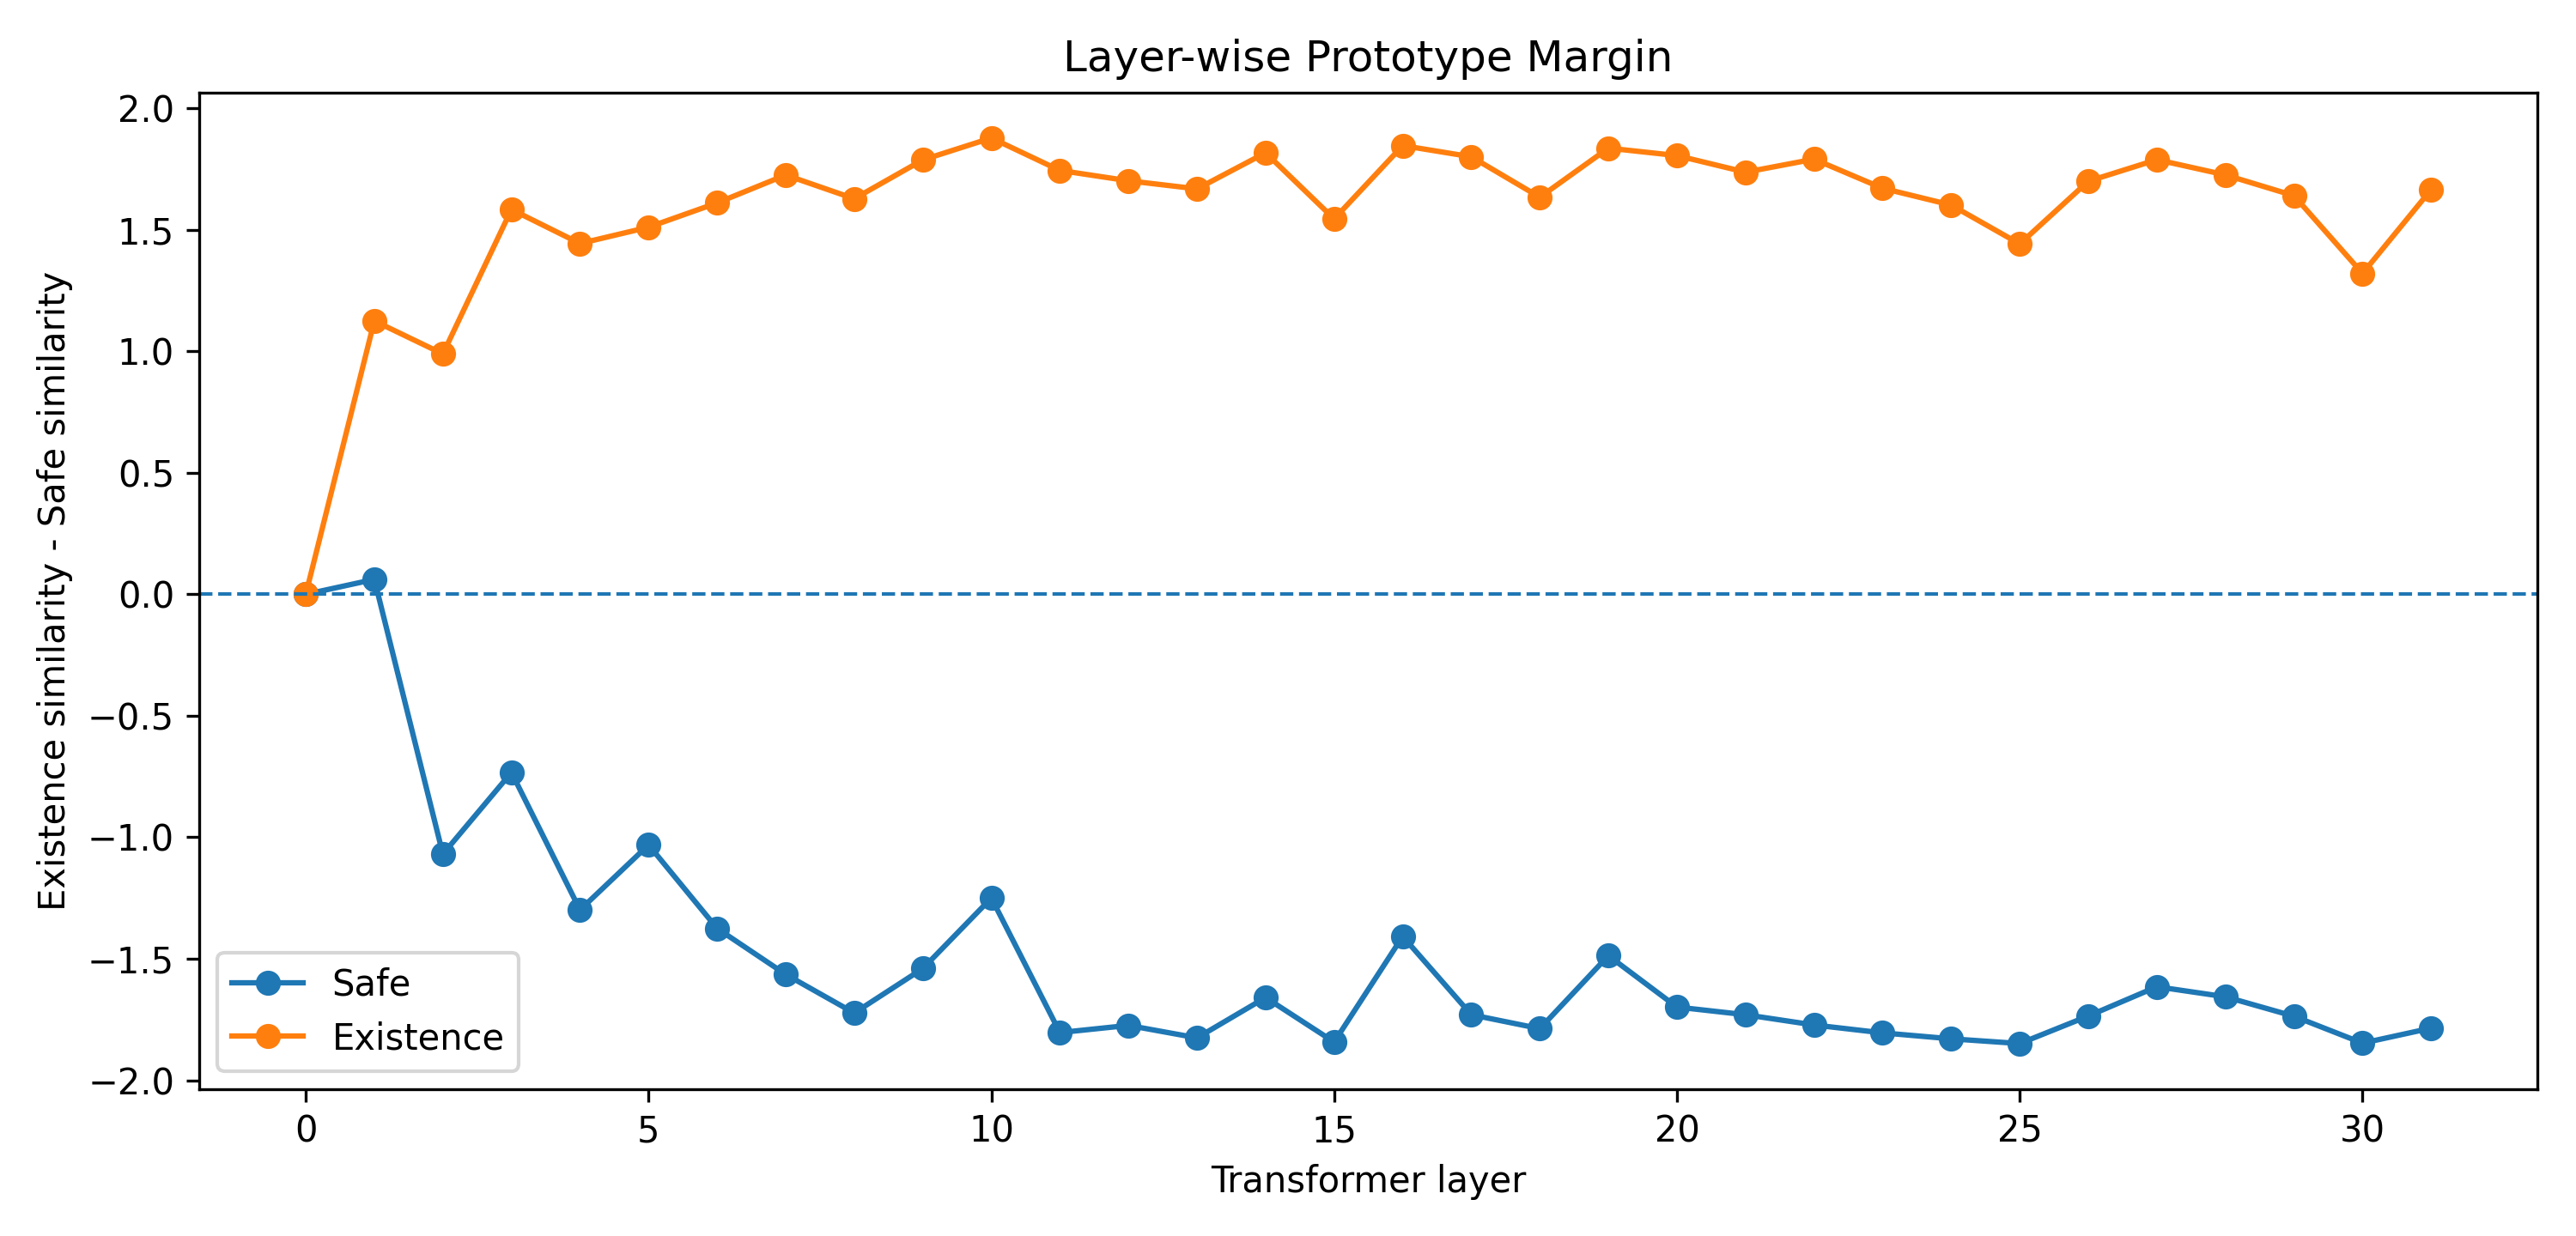
\includegraphics[width=0.48\linewidth]{figures/layerwise_margin.png}
\hfill
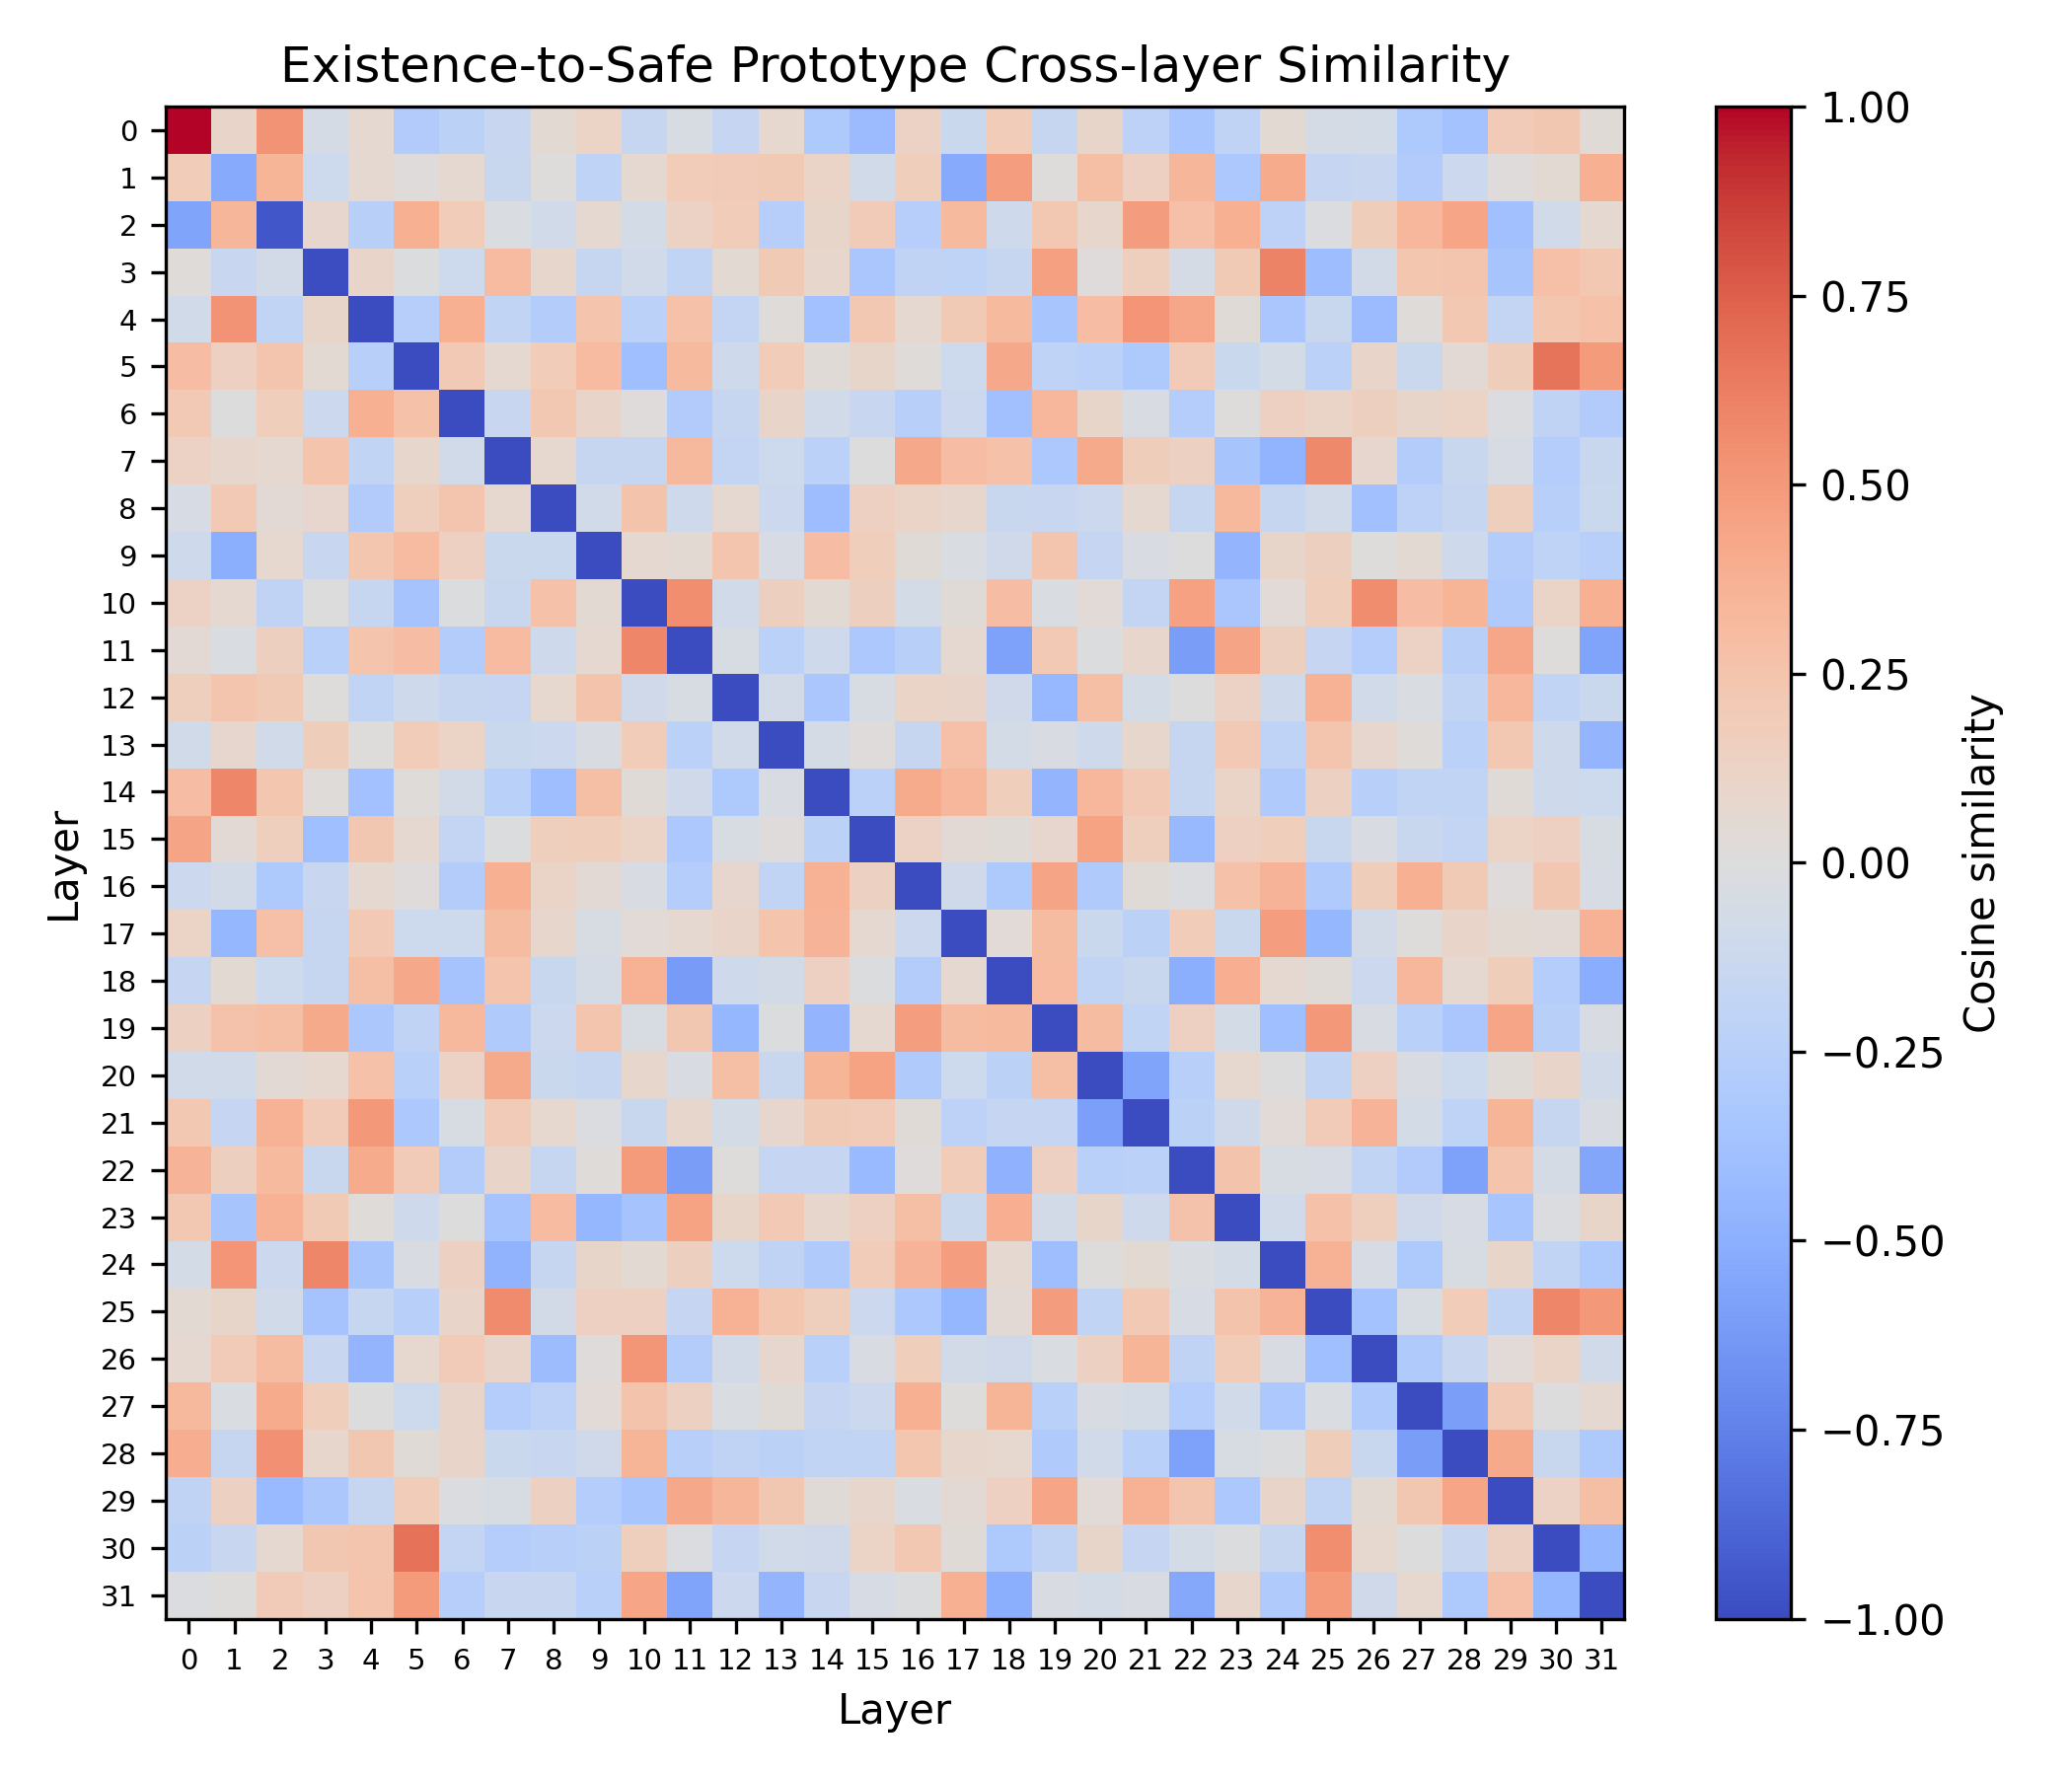
\includegraphics[width=0.48\linewidth]{figures/cross_layer_similarity.png}
\caption{Concept separation analysis. Left: layer-wise prototype margin between Safe and Existence concepts. Right: cross-layer prototype similarity matrix.}
\label{fig:concept_separation}
\end{figure}

As shown in Figure~\ref{fig:concept_separation}, Safe and Existence concepts begin to separate after approximately the third transformer layer, and the margin converges around the eighth layer. This indicates that the learned prototypes capture distinct representation patterns associated with hallucination behavior.

The cross-layer similarity matrix further shows strong diagonal patterns, suggesting that each layer learns a stable and distinct concept representation. Together, these results indicate consistent concept separation throughout the network.

\paragraph{Stronger Signals in Deeper Layers}

We further analyze prototype activation distributions across early, middle, and late transformer layers.

\begin{figure}[t]
\centering
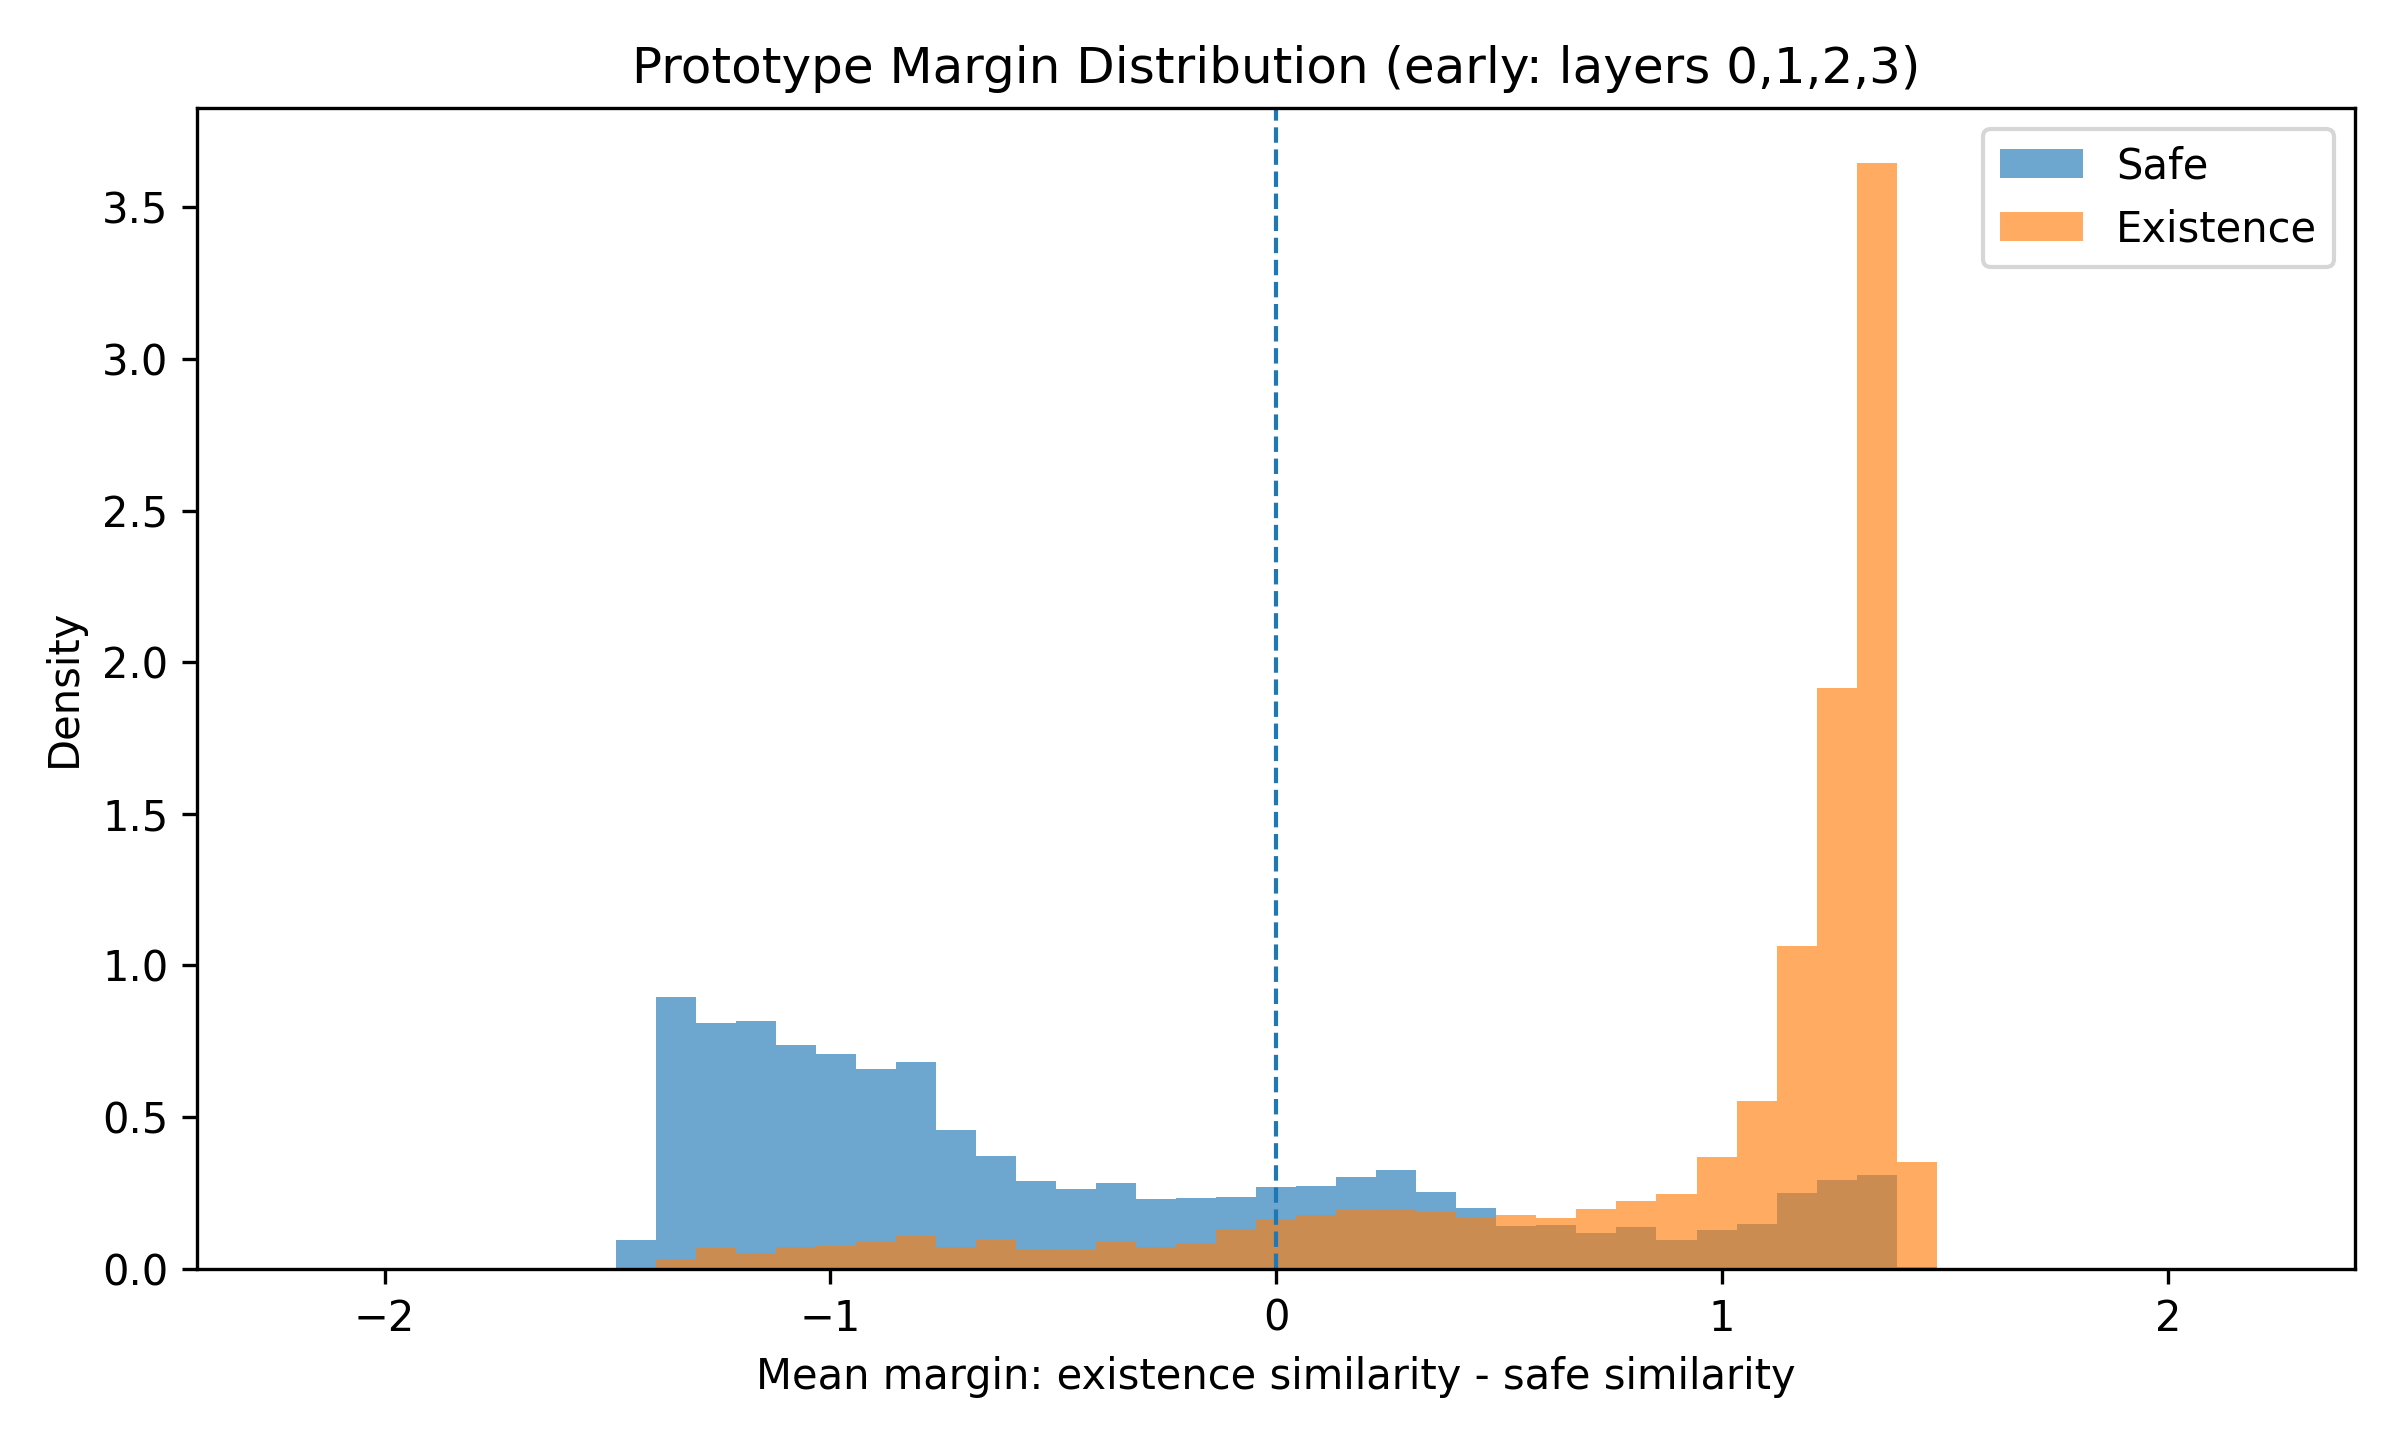
\includegraphics[width=0.32\linewidth]{figures/distribution_early.png}
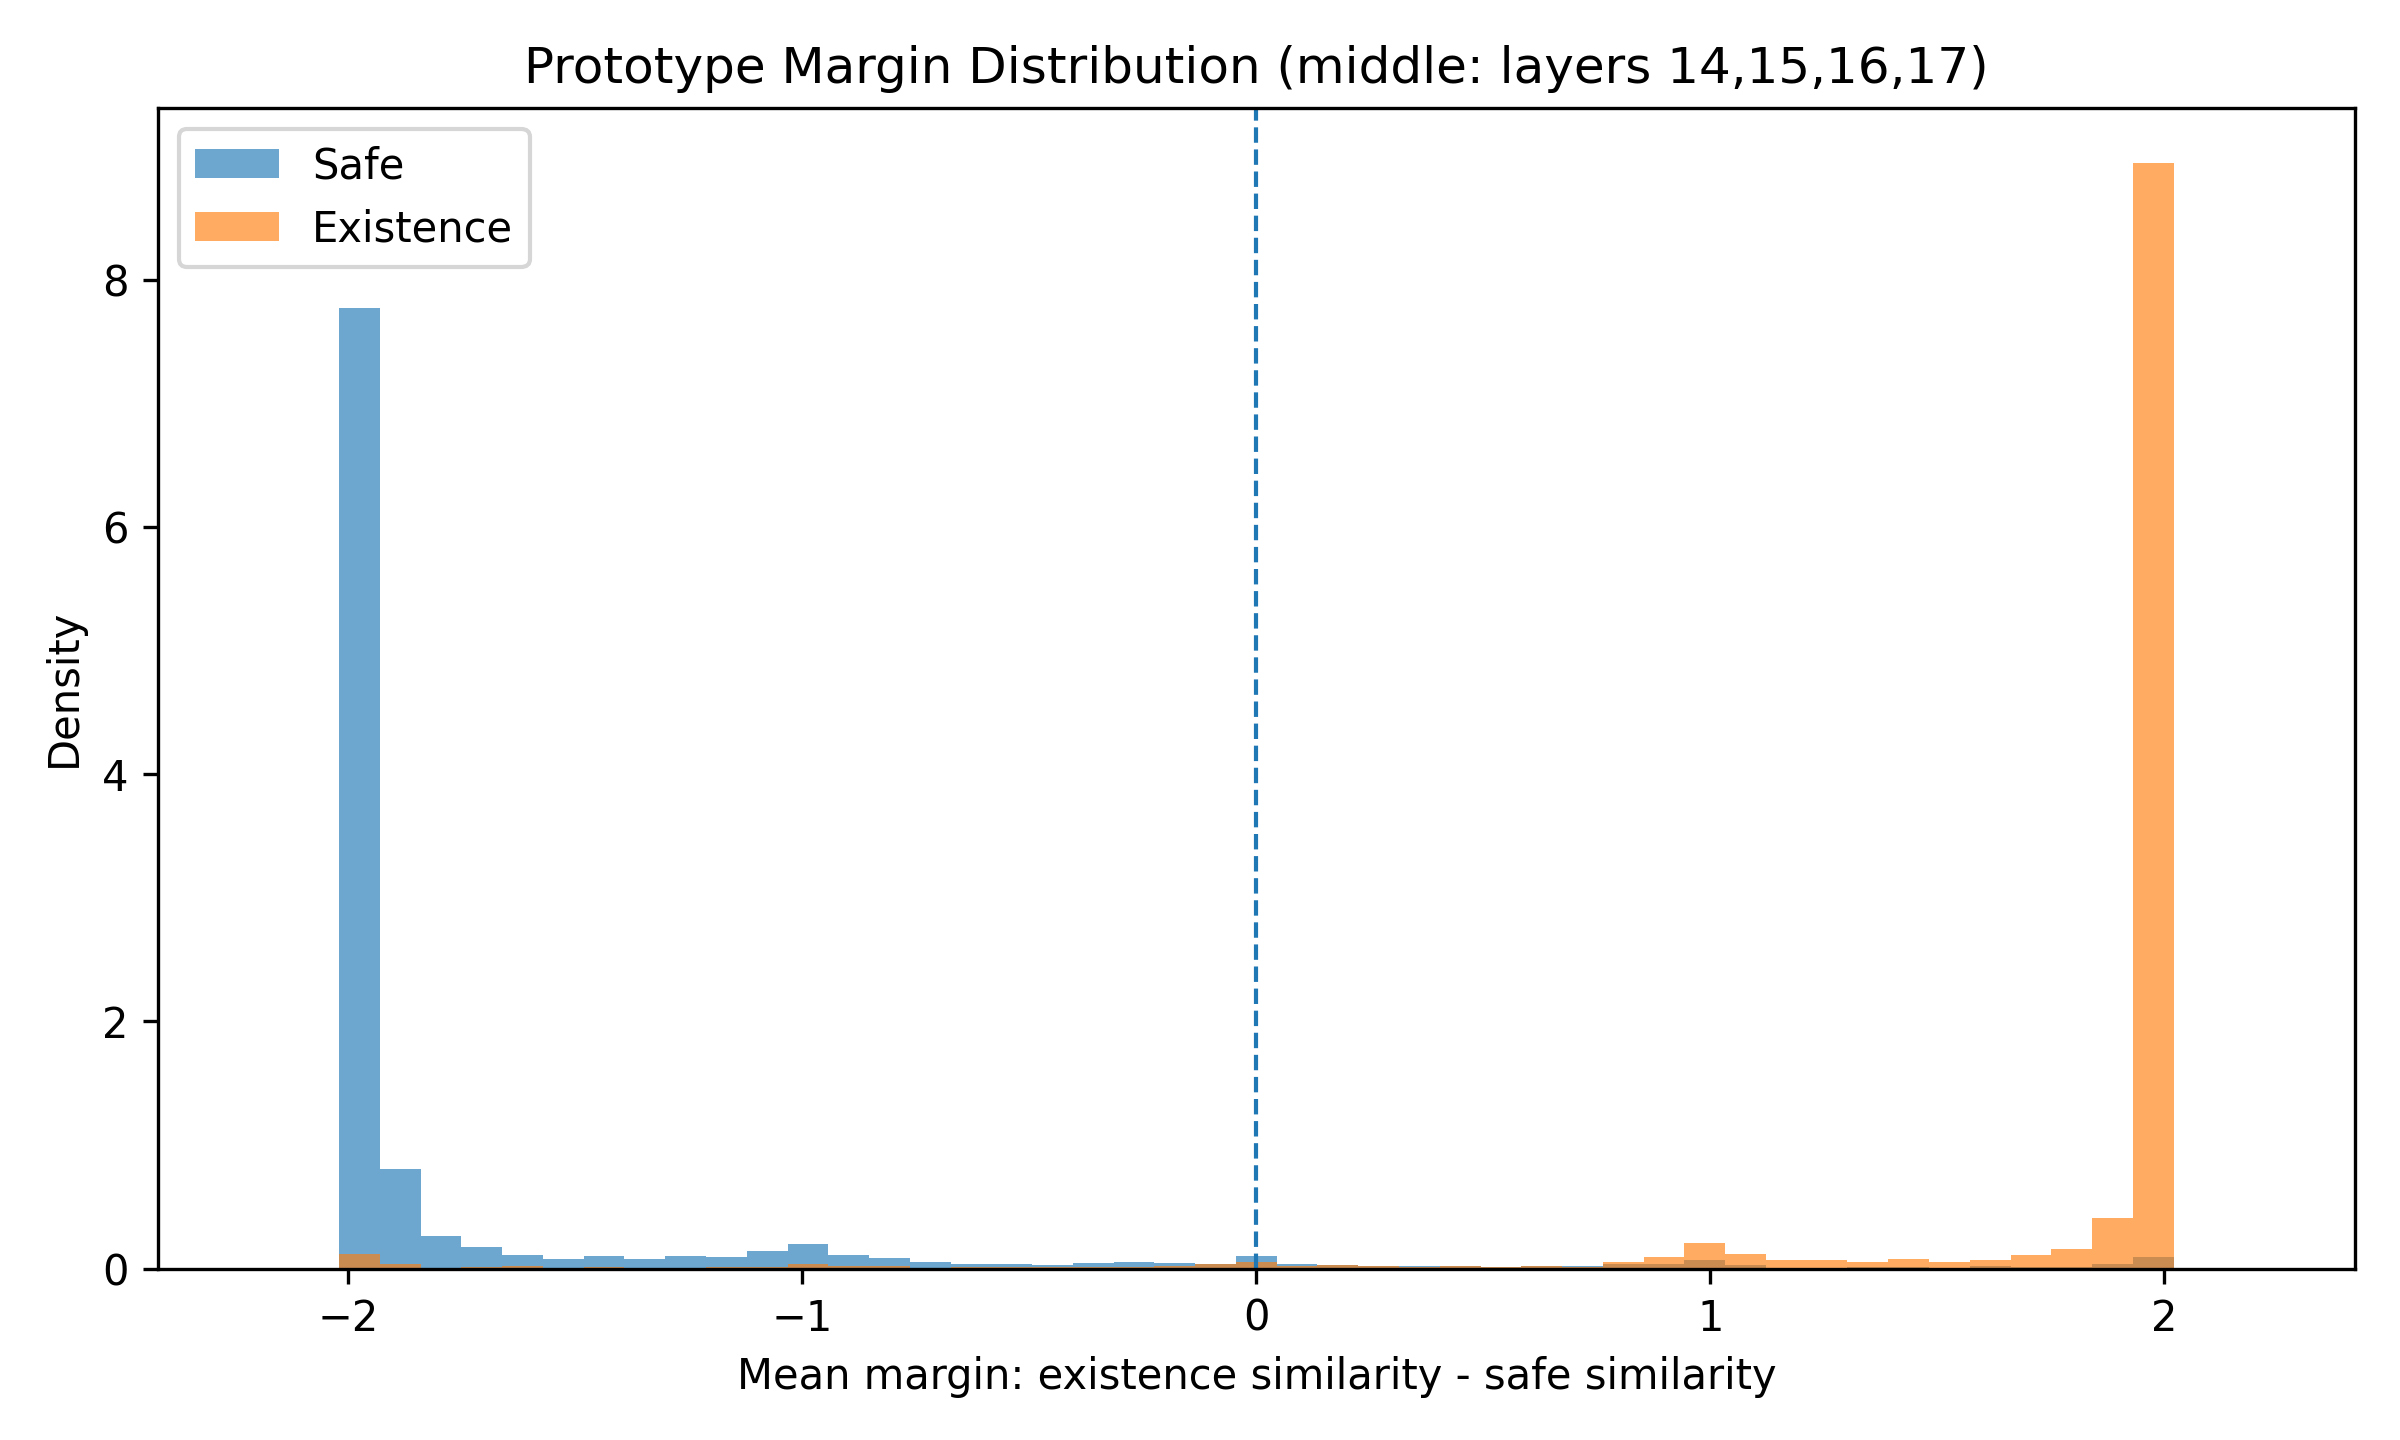
\includegraphics[width=0.32\linewidth]{figures/distribution_middle.png}
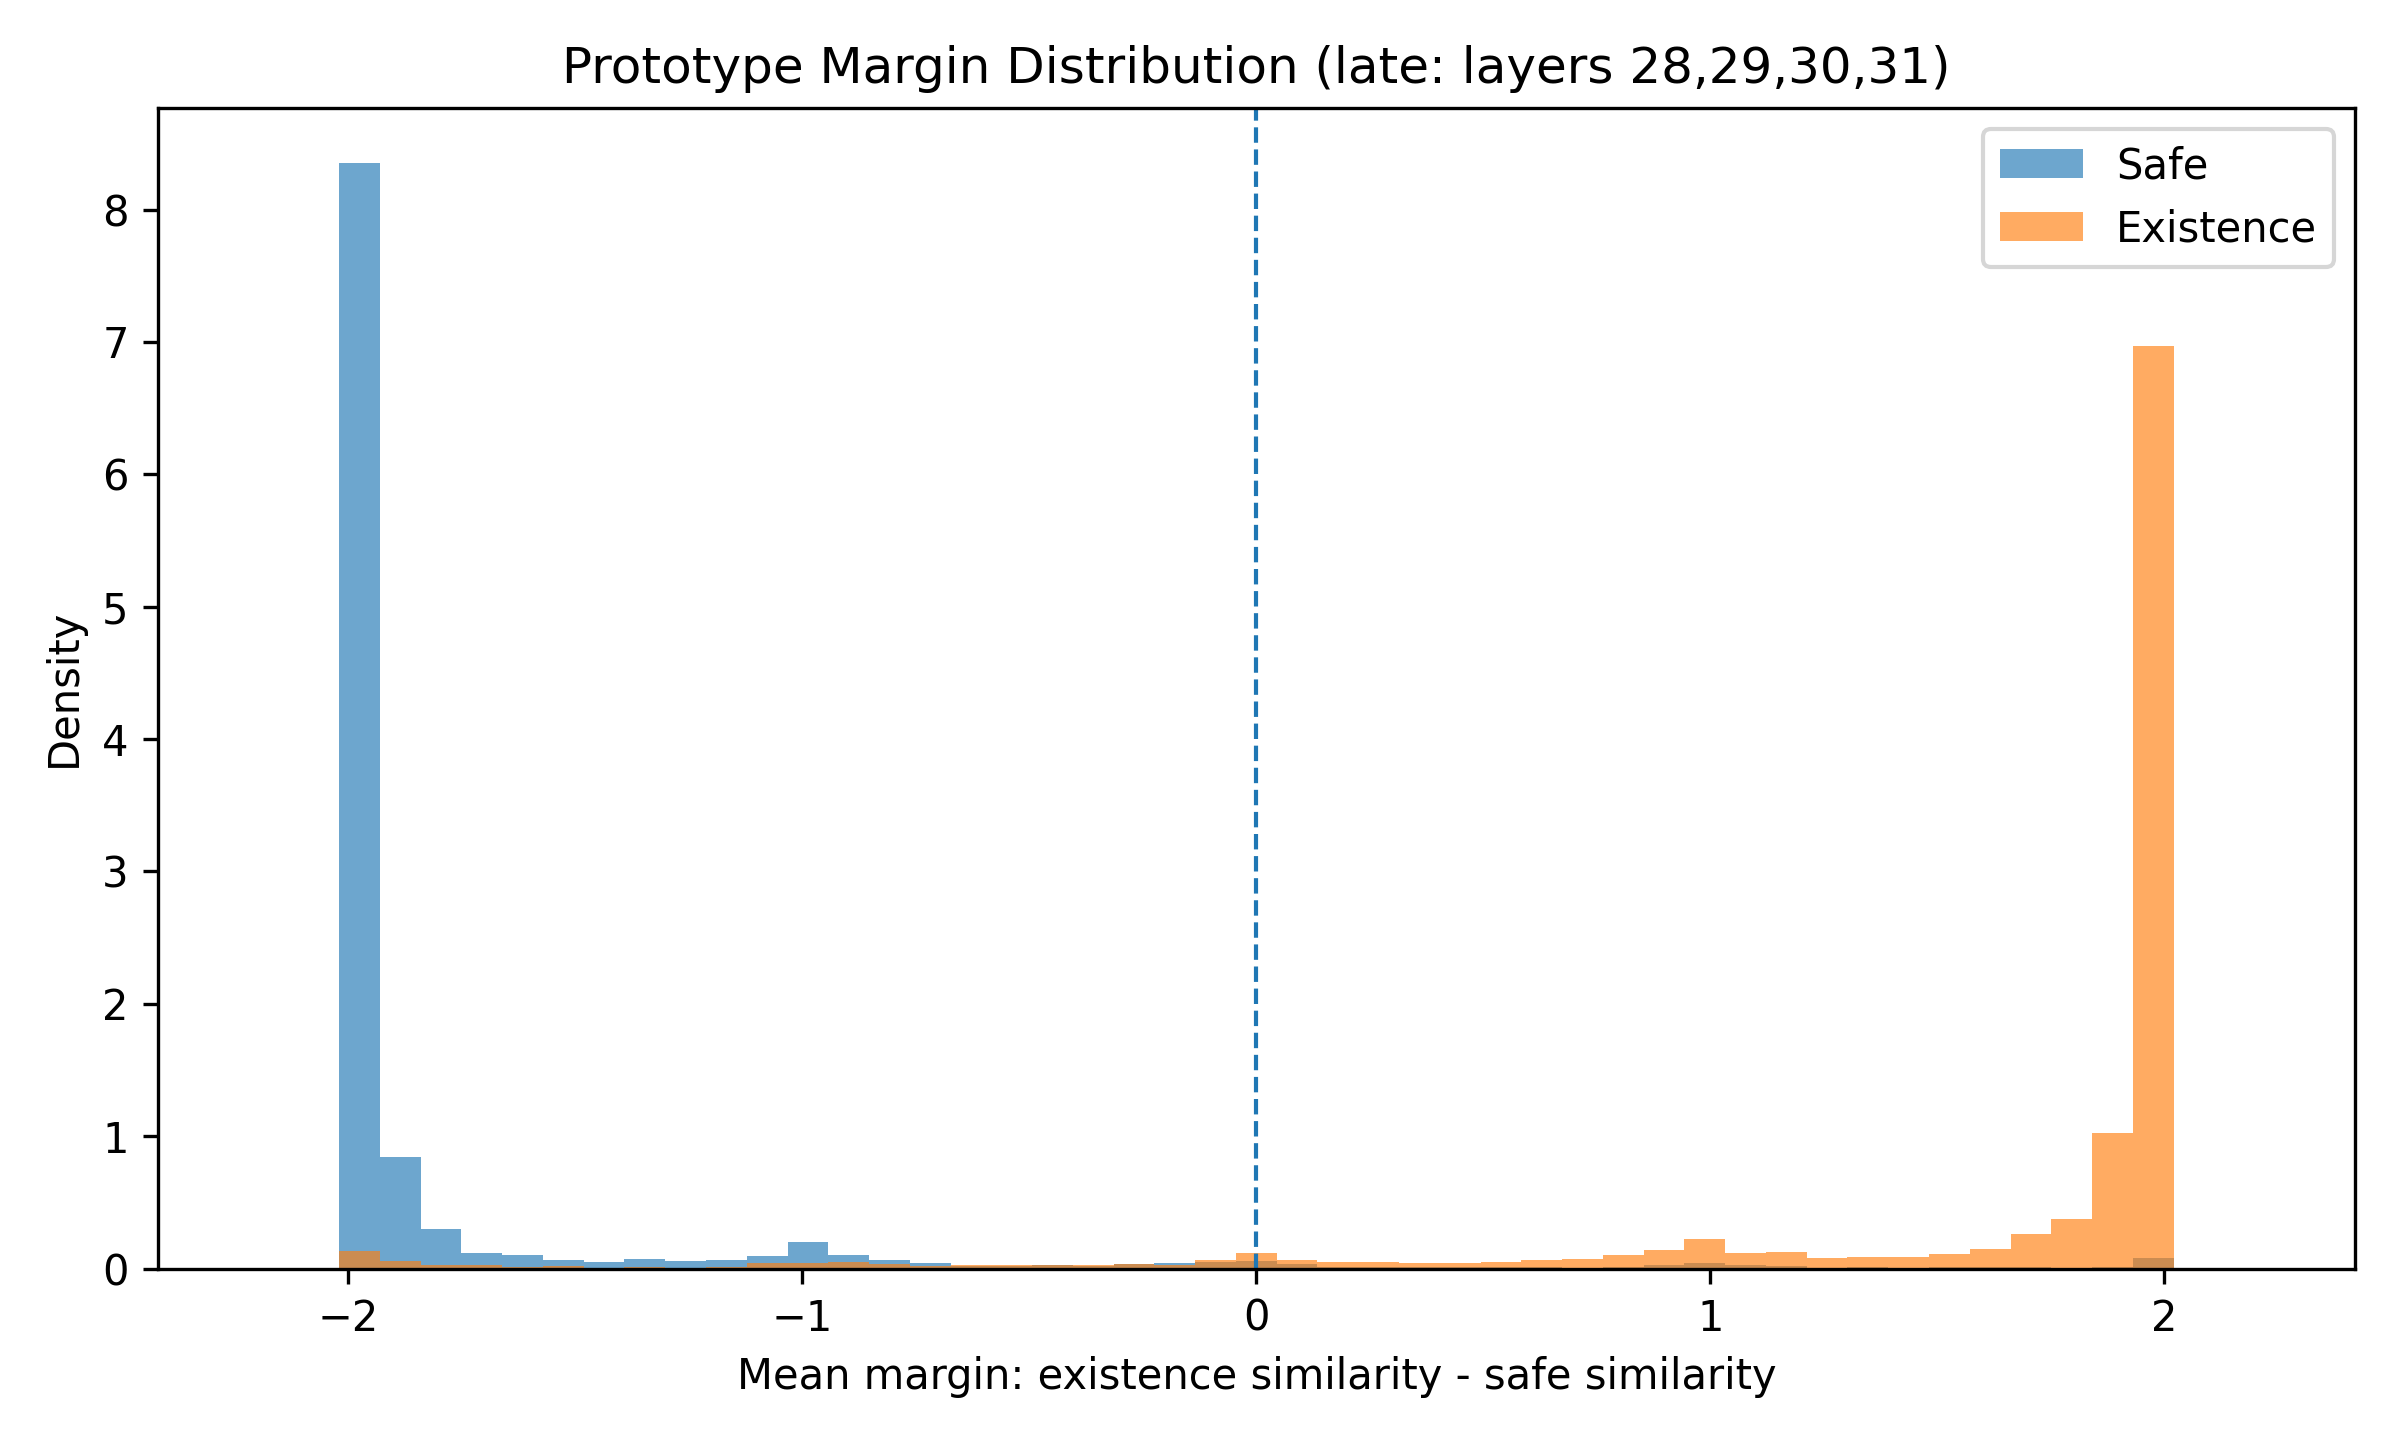
\includegraphics[width=0.32\linewidth]{figures/distribution_late.png}
\caption{Prototype activation distributions across transformer layers.}
\label{fig:distribution}
\end{figure}

Figure~\ref{fig:distribution} shows substantial overlap between Safe and Existence concepts in early layers. However, the separation becomes increasingly clear in middle and deeper layers.

This trend suggests that hallucination-related information becomes progressively more distinguishable as representations move toward higher semantic abstraction levels.



\subsubsection{Limitation}

Although the proposed framework provides meaningful concept-level interpretations of hallucination-related representations, several limitations remain.

\begin{figure}[t]
\centering
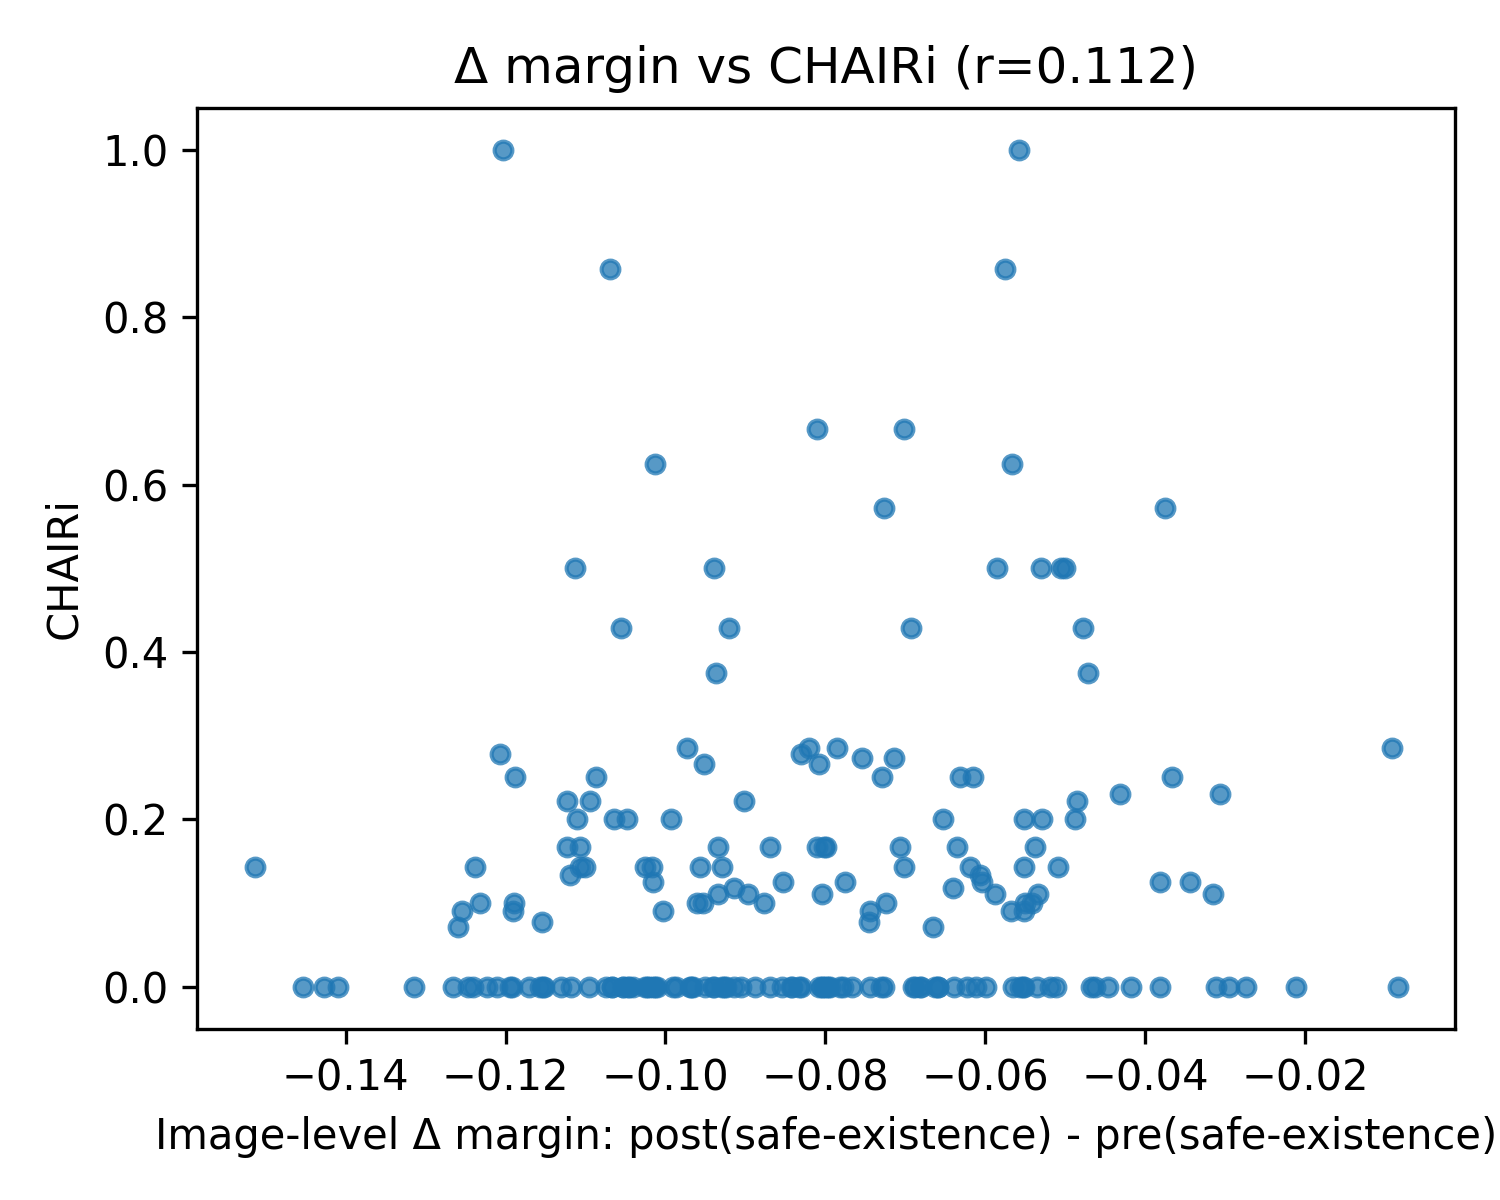
\includegraphics[width=0.48\linewidth]{figures/delta_vs_chairi.png}
\hfill
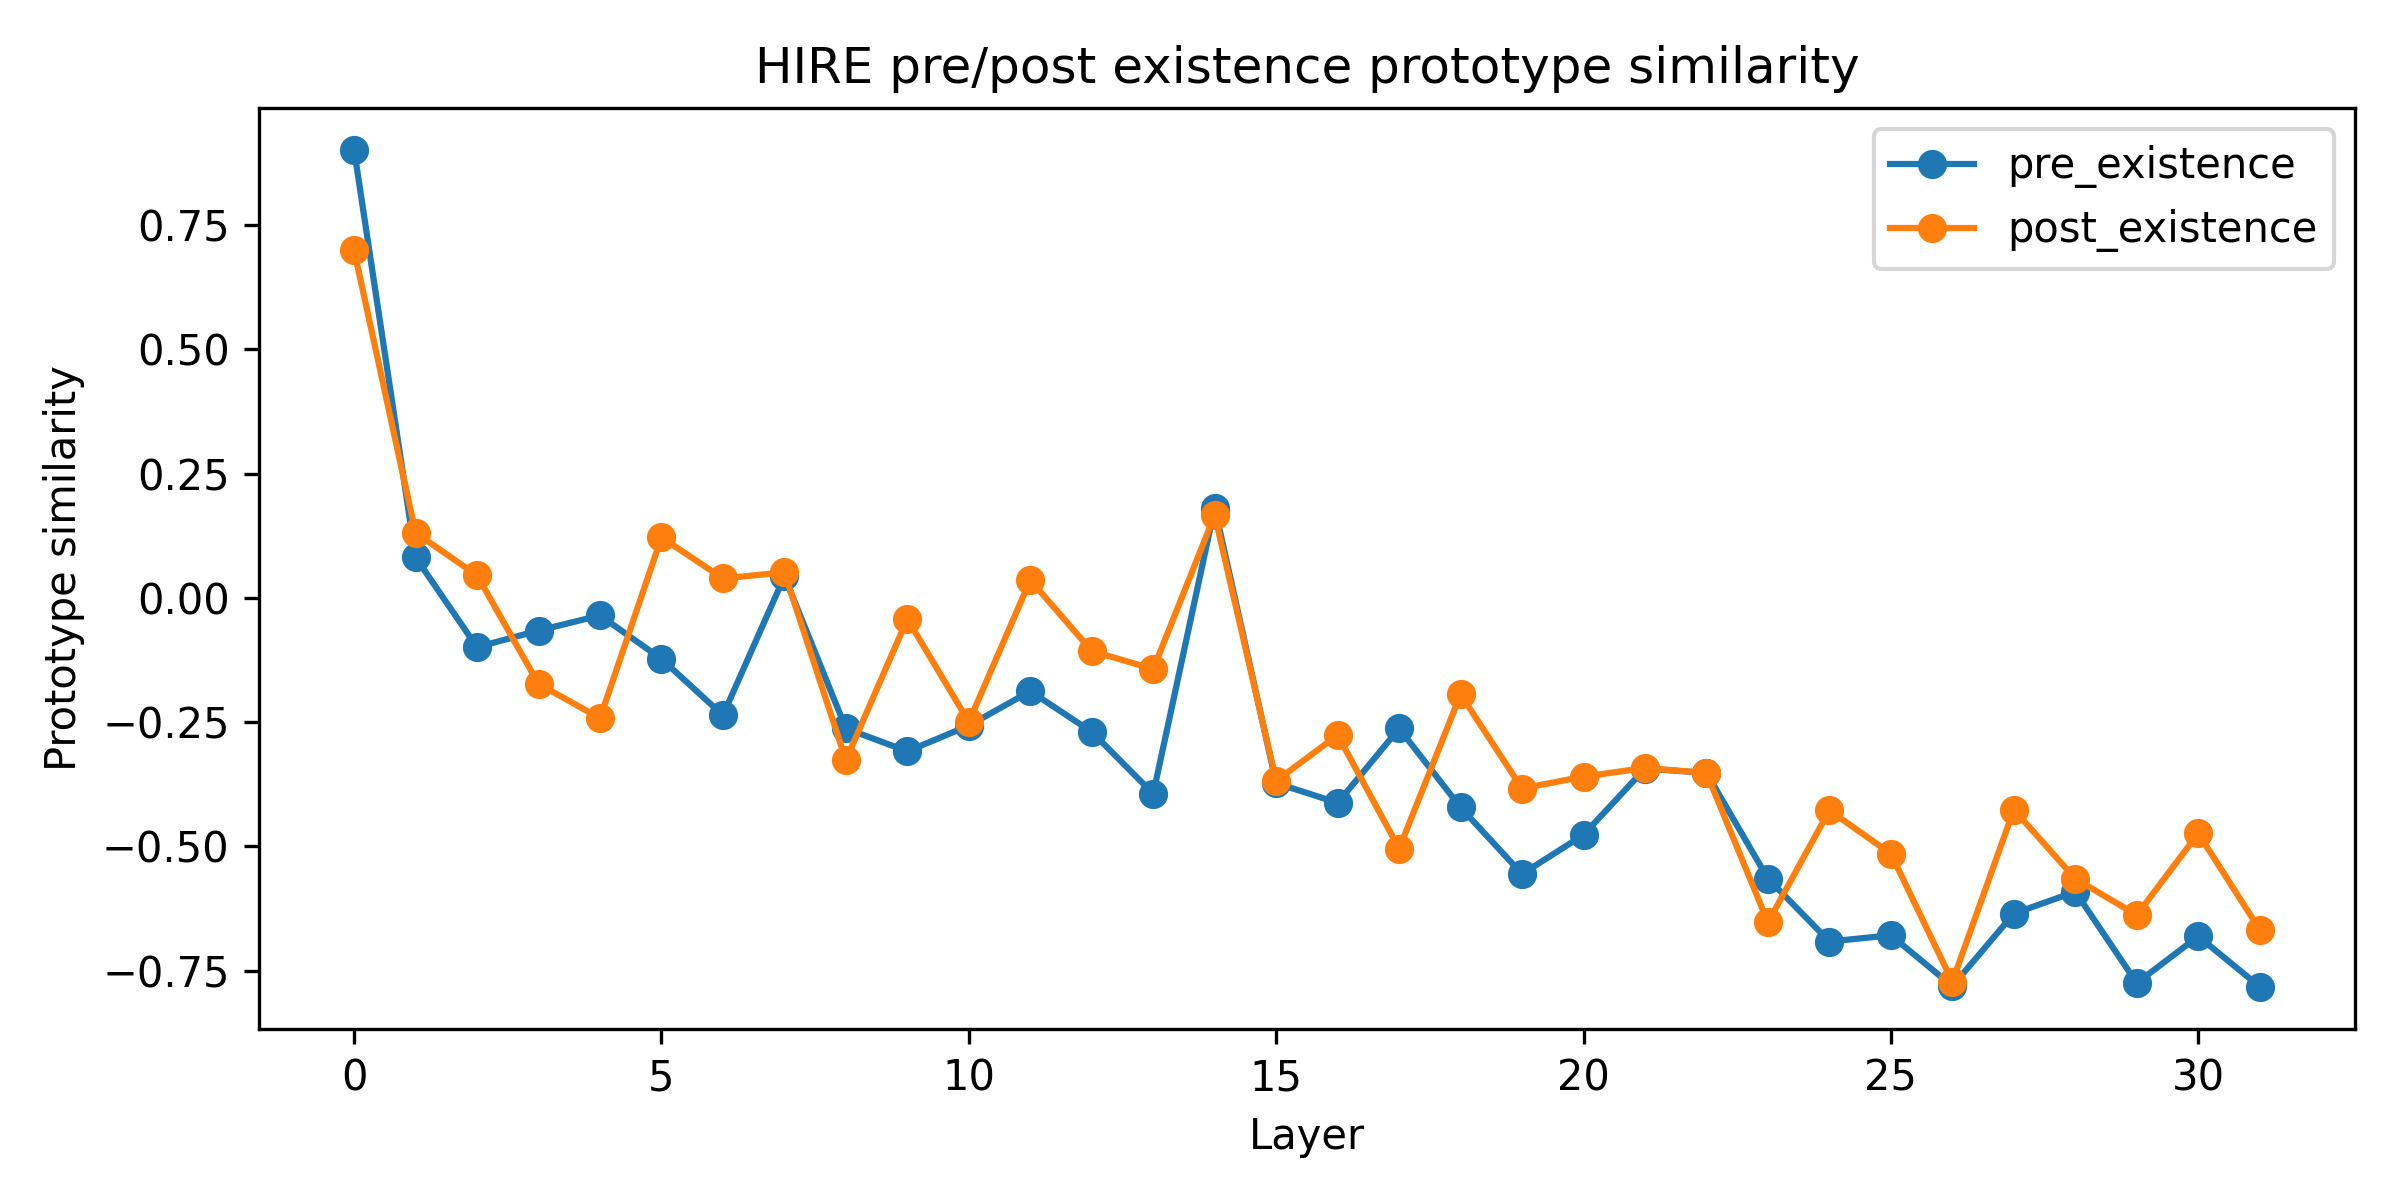
\includegraphics[width=0.48\linewidth]{figures/pre_post_existence_curve.png}
\caption{Limitations of the proposed framework. Left: relationship between concept activation changes and CHAIRi scores. Right: layer-wise Existence concept activations.}
\label{fig:limitation_analysis}
\end{figure}

As shown in Figure~\ref{fig:limitation_analysis}, concept activations exhibit only moderate correlations with hallucination metrics. Furthermore, although Existence activations become increasingly pronounced in deeper layers, the learned concepts are not directly aligned with HIRE's editing objective.

We believe this limitation arises because our framework focuses exclusively on Existence hallucinations, whereas HIRE addresses multiple hallucination categories simultaneously. Consequently, concept activations capture hallucination-related characteristics but remain weakly connected to actual hallucination mitigation performance.

The proposed framework also introduces additional computational overhead due to layer-wise representation extraction and prototype similarity computation.

\begin{table}[t]
\centering
\caption{Inference overhead introduced by the layer-wise CBM module.}
\begin{tabular}{lccc}
\hline
Model & Runtime (s) & With CBM (s) & Overhead \\
\hline
LLaVA & 60 & 352 & 5.87$\times$ \\
HIRE & 139 & 1212 & 8.72$\times$ \\
\hline
\end{tabular}
\label{tab:runtime_results}
\end{table}

As shown in Table~\ref{tab:runtime_results}, the additional analysis module increases inference time by approximately $5.9\times$ to $8.7\times$.

Future work will focus on extending the concept space beyond Existence hallucinations and integrating concept information directly into representation editing frameworks.






